\documentclass[11pt]{article}
\input{../../notes-style.tex}

\title{CS 300 -- Chapter 11 Notes\\\large B-Trees}
\author{Jose de Lima}
\date{\today}

\begin{document}
\maketitle

\begin{ideabox}
\textbf{Why B-trees exist.} AVL and red-black trees (ch.\ 9) optimize for in-memory comparisons: each node holds one key and two children. But when your tree doesn't fit in RAM -- when it lives on disk or across a network -- a binary tree is a disaster. Each node traversal is a separate I/O operation. A tree of a billion keys is $\log_2 10^9 \approx 30$ levels deep; that's 30 disk seeks per lookup at roughly 10ms each = 300ms per query. A B-tree of the same size is $\log_{100} 10^9 \approx 4.5$ levels deep. Fatter nodes, fewer levels, fewer I/Os. \emph{B-trees are what happens when you let cache lines or disk blocks dictate your node size.}
\end{ideabox}

\section{11.1 B-tree Structure}

\subsection*{The definition}

\begin{defnbox}
\textbf{B-tree of order $K$.} A search tree where every node holds up to $K-1$ keys and up to $K$ children. Subject to:
\begin{itemize}[leftmargin=*]
    \item All keys in a node are stored in sorted order.
    \item An internal node with $n$ keys has exactly $n+1$ children.
    \item Between two adjacent keys, the child subtree holds keys strictly between them; outside the first or last key, the outer subtrees hold keys strictly less / greater.
    \item All leaves sit at the same depth. (This is the balance condition.)
    \item All keys are distinct.
\end{itemize}
\end{defnbox}

\begin{notebox}
Different textbooks use subtly different definitions of ``order'' -- some count maximum children ($K$), some count maximum keys ($K-1$), some use a \emph{minimum} degree $t$ with $t-1$ to $2t-1$ keys per node. These notes use ``order $K$ = max children.'' Translate carefully if you cross-reference CLRS or Knuth.
\end{notebox}

\subsection*{The 2-3-4 tree -- a B-tree of order 4}

Order-4 B-trees are the standard teaching example. A node holds:
\begin{itemize}[leftmargin=*]
    \item 1, 2, or 3 keys -- called \textbf{2-node}, \textbf{3-node}, or \textbf{4-node}.
    \item Correspondingly 2, 3, or 4 children (for internal nodes).
\end{itemize}

A common convention labels node keys as $A$, $B$, $C$ and children as \texttt{left}, \texttt{middle1}, \texttt{middle2}, \texttt{right}:

\begin{center}
\begin{tabular}{lll}
\hline
Node type & Keys used & Children used \\
\hline
2-node & $A$ & \texttt{left}, \texttt{middle1} \\
3-node & $A, B$ & \texttt{left}, \texttt{middle1}, \texttt{middle2} \\
4-node (full) & $A, B, C$ & \texttt{left}, \texttt{middle1}, \texttt{middle2}, \texttt{right} \\
\hline
\end{tabular}
\end{center}

\begin{ideabox}
2-3-4 trees are a finger exercise. Real B-trees in databases use orders in the hundreds or thousands -- typically whatever fits in one disk page (4KB--16KB) or one L2 cache line (a few hundred integers). The \emph{algorithms} are identical to the order-4 version; only the array sizes change.
\end{ideabox}

\subsection*{C++ node skeleton}

\begin{lstlisting}[basicstyle=\ttfamily\small,frame=single]
template<int Order>   // e.g. Order=4 for 2-3-4 trees
struct BTreeNode {
    int numKeys = 0;
    int keys[Order - 1];
    BTreeNode* children[Order] = {};     // null for leaves
    BTreeNode* parent = nullptr;

    bool isLeaf() const { return children[0] == nullptr; }
    bool isFull() const { return numKeys == Order - 1; }
};
\end{lstlisting}

\subsection*{Height analysis}

A B-tree of order $K$ with $n$ keys has height $h = O(\log_K n)$. For $K = 100$ and $n = 10^9$, that's $\log_{100} 10^9 \approx 4.5$ -- roughly 5 node accesses per lookup. Contrast with a binary tree's $\log_2 10^9 \approx 30$.

That factor-of-six reduction is the whole point. On disk it translates directly to query latency.

\begin{examplebox}
\textbf{Where B-trees actually live.}
\begin{itemize}[leftmargin=*]
    \item \textbf{Database indexes}: MySQL (InnoDB), PostgreSQL, SQL Server, Oracle all use B+ trees (a B-tree variant) for their default index structures.
    \item \textbf{Filesystems}: ext4, NTFS, HFS+, APFS, Btrfs (the ``B'' is for B-tree), XFS -- all B-tree-based for directory and extent management.
    \item \textbf{Key-value stores}: BoltDB, LMDB use B+ trees.
    \item \textbf{Version control}: Git's packfile index uses a B-tree-like structure for fast object lookup.
\end{itemize}
You won't ``implement a B-tree for production'' very often, but you'll read about them in every system's architecture doc.
\end{examplebox}

\section{11.2 Search}

\subsection*{The algorithm}

B-tree search is binary search \emph{within} a node combined with tree descent. At each node:
\begin{enumerate}[leftmargin=*]
    \item Linear-scan (or binary-search, for larger orders) the node's keys for the target.
    \item If found, return the node.
    \item Otherwise, find the child whose key range contains the target, and recurse.
\end{enumerate}

For the 2-3-4 case, the child selection reduces to a short comparison chain:

\begin{center}
\begin{tabular}{ll}
\hline
Condition & Descend to \\
\hline
key $<$ node.A & \texttt{left} \\
node has 1 key, or key $<$ node.B & \texttt{middle1} \\
node has 2 keys, or key $<$ node.C & \texttt{middle2} \\
otherwise & \texttt{right} \\
\hline
\end{tabular}
\end{center}

\begin{lstlisting}[basicstyle=\ttfamily\small,frame=single]
BTreeNode* btreeSearch(BTreeNode* node, int key) {
    if (!node) return nullptr;

    // Check keys in this node.
    if (node->numKeys >= 1 && node->keys[0] == key) return node;
    if (node->numKeys >= 2 && node->keys[1] == key) return node;
    if (node->numKeys >= 3 && node->keys[2] == key) return node;

    // Descend to the appropriate child.
    if (key < node->keys[0])
        return btreeSearch(node->children[0], key);     // left
    if (node->numKeys == 1 || key < node->keys[1])
        return btreeSearch(node->children[1], key);     // middle1
    if (node->numKeys == 2 || key < node->keys[2])
        return btreeSearch(node->children[2], key);     // middle2
    return btreeSearch(node->children[3], key);         // right
}
\end{lstlisting}

\subsection*{Cost}

\begin{itemize}[leftmargin=*]
    \item $O(\log_K n)$ node accesses (one per level).
    \item $O(K)$ comparisons \emph{per node} -- linear scan over the keys. With binary search, that's $O(\log K)$.
    \item Total: $O(\log_K n \cdot \log K) = O(\log n)$. Same Big-O as a balanced binary tree, but with a \emph{much} smaller constant factor in number of node accesses.
\end{itemize}

\begin{ideabox}
Big-O hides the real win. A binary tree and a B-tree both do $O(\log n)$ comparisons, but the B-tree does them with one-tenth the \emph{pointer dereferences}. When each pointer dereference is a cache miss (or a disk seek), that's a 10$\times$ speedup, even though the asymptotic complexity is identical.
\end{ideabox}

\section{11.3 Insertion}

\subsection*{The big picture}

New keys always go into leaf nodes. The challenge: leaves might already be full. Strategy:

\begin{ideabox}
\textbf{Preemptive split.} As we descend from the root to the target leaf, \emph{split any full node we encounter along the way}. This guarantees the target leaf has room. Splits never cascade up, because every ancestor we visited is already non-full (we would have split it if not).
\end{ideabox}

\subsection*{The split operation}

A full node (with its maximum $K-1$ keys) is split into two nodes of $(K/2 - 1)$ keys each, and the middle key is promoted to the parent. For 2-3-4 trees:

\begin{center}
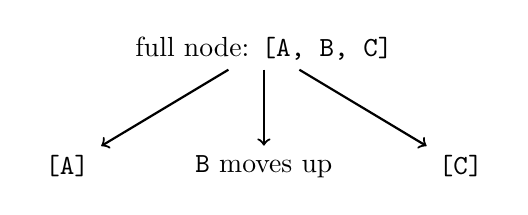
\begin{tikzpicture}[every node/.style={minimum width=1cm, minimum height=0.5cm}]
\node (src) at (0, 1.5) {full node: \texttt{[A, B, C]}};
\node (a) at (-2.5, 0) {\texttt{[A]}};
\node (parent) at (0, 0) {\texttt{B} moves up};
\node (c) at (2.5, 0) {\texttt{[C]}};
\draw[->, thick] (src) -- (a);
\draw[->, thick] (src) -- (parent);
\draw[->, thick] (src) -- (c);
\end{tikzpicture}
\end{center}

Keys $A$ and $C$ become two new sibling nodes; key $B$ moves into the parent, with pointers to the new siblings. The parent must have room (thanks to preemptive split).

\begin{lstlisting}[basicstyle=\ttfamily\small,frame=single]
BTreeNode* btreeSplit(BTree& t, BTreeNode* node) {
    if (!node->isFull()) return nullptr;
    BTreeNode* parent = node->parent;
    BTreeNode* left  = new BTreeNode{1, {node->keys[0]},
                                     {node->children[0], node->children[1]},
                                     parent};
    BTreeNode* right = new BTreeNode{1, {node->keys[2]},
                                     {node->children[2], node->children[3]},
                                     parent};

    if (parent) {
        btreeInsertKeyWithChildren(parent, node->keys[1], left, right);
    } else {
        parent = new BTreeNode{1, {node->keys[1]}, {left, right}, nullptr};
        t.root = parent;
        left->parent = right->parent = parent;
    }
    return parent;
}
\end{lstlisting}

\subsection*{Special case: splitting the root}

When the root itself is full and we start inserting, the split creates a brand-new root with a single key. \textbf{This is the only way a B-tree grows in height.} Every other operation happens at the leaf level or via splits that push keys sideways to a non-full ancestor.

\begin{ideabox}
B-trees grow from the \emph{top} (via root splits), unlike binary search trees which grow from the bottom. That's why all leaves stay at the same depth -- depth increases uniformly when the root splits.
\end{ideabox}

\subsection*{Insert into a leaf}

Once we've descended (splitting along the way) to the target leaf, the leaf is guaranteed non-full. Insert the new key in sorted position:

\begin{center}
\begin{tabular}{ll}
\hline
Condition (non-full leaf) & Action \\
\hline
key equals existing key & no-op (duplicates forbidden) \\
key $<$ node.A & shift existing keys right, place new key at $A$ \\
key $<$ node.B (or no $B$) & shift $B \to C$ if needed, place new key at $B$ \\
otherwise & place new key at $C$ \\
\hline
\end{tabular}
\end{center}

\subsection*{The full insert}

\begin{lstlisting}[basicstyle=\ttfamily\small,frame=single]
BTreeNode* btreeInsert(BTreeNode* node, int key) {
    if (containsKey(node, key)) return nullptr;   // duplicates rejected

    if (node->isFull()) node = btreeSplit(node);  // preemptive split

    if (!node->isLeaf()) {
        BTreeNode* child = btreeChildForKey(node, key);
        return btreeInsert(child, key);
    }
    btreeInsertIntoLeaf(node, key);
    return node;
}
\end{lstlisting}

\subsection*{Cost}

\begin{itemize}[leftmargin=*]
    \item Descent: $O(\log_K n)$ levels.
    \item At each level: at most one split, $O(K)$ work.
    \item Total: $O(K \log_K n)$. For fixed $K$, that's $O(\log n)$.
\end{itemize}

\begin{warnbox}
\textbf{The ``lazy'' alternative.} Instead of preemptive split, you can insert into the leaf first, and \emph{then} split if the leaf became full -- cascading splits upward. That's the classical Knuth algorithm and is slightly more space-efficient (nodes can fill up more before being split). Preemptive split is preferred in teaching because it's a single downward pass -- no recursion up the tree.
\end{warnbox}

\section{11.4 Rotations and Fusion}

Removal is the hard half of any balanced tree. For B-trees, the two tools are \textbf{rotation} (borrow a key from a sibling) and \textbf{fusion} (merge three nodes into one -- the inverse of split).

\subsection*{Rotation}

\begin{defnbox}
\textbf{Rotation (B-tree sense).} Move one key from a source node, \emph{through the parent}, into a sibling. The source loses a key, the sibling gains a key, and the parent key that was between them is swapped out for a key from the source.
\end{defnbox}

\begin{ideabox}
This is \emph{not} the same as the AVL/red-black rotation. AVL rotations re-parent subtrees to restore a height balance. B-tree rotations \textbf{redistribute keys across sibling nodes} -- the tree shape doesn't change, only which key lives in which node.
\end{ideabox}

\subsection*{Right rotation on \texttt{node}}

Takes a key from \texttt{node}'s left sibling, moves the parent separator key into \texttt{node}, and pushes the left sibling's rightmost key up to fill the separator slot. Result: the left sibling loses one key, \texttt{node} gains one.

\subsection*{Left rotation on \texttt{node}}

Mirror image: takes a key from \texttt{node}'s right sibling.

\begin{lstlisting}[basicstyle=\ttfamily\small,frame=single]
// Illustrative form. A "rotation on node X" in this context means
// "give X one more key by borrowing from a sibling through the parent."
void btreeRotateLeft(BTreeNode* node) {
    BTreeNode* leftSib = getLeftSibling(node);
    int parentKey = getParentKeyLeftOfChild(node->parent, node);
    addKeyAndChild(leftSib, parentKey, node->children[0]);
    setParentKeyLeftOfChild(node->parent, node, node->keys[0]);
    removeKey(node, 0);
}
\end{lstlisting}

\subsection*{Fusion}

\begin{defnbox}
\textbf{Fusion.} Merge a parent separator key with two single-key adjacent siblings into one fused 3-key node. \emph{The inverse of split.}
\end{defnbox}

\begin{center}
\begin{tabular}{lll}
Before fusion & $\to$ & After fusion \\
\texttt{[L]} $\cdot$ (parent sep $M$) $\cdot$ \texttt{[R]} & $\to$ & \texttt{[L, M, R]} \\
\end{tabular}
\end{center}

The parent loses a key (and a child pointer); the fused node has three keys. Fusion is used when neither sibling has a spare key to rotate.

\subsection*{Root fusion -- a special case}

When the root has 1 key and both its children have 1 key each, no rotation is possible and ordinary fusion would empty the parent. Instead, the three keys are combined into a \emph{new root} of three keys, and the tree shrinks in height by 1:

\begin{ideabox}
Root fusion is the only way a B-tree shrinks in height, mirroring how root split is the only way it grows. Every other operation happens at leaf level or via local restructuring.
\end{ideabox}

\subsection*{Visualizing split vs.\ fusion}

\begin{center}
\begin{tabular}{lcc}
\hline
Operation & Effect on height & Inverse of \\
\hline
Root split & +1 & Root fusion \\
Internal split & 0 & Internal fusion \\
Right rotation & 0 & Left rotation (roughly) \\
\hline
\end{tabular}
\end{center}

The symmetry is beautiful: \emph{every modification to a B-tree is either a rotation (constant-cost redistribution) or a split/fuse (constant-cost restructuring)}. Both are strictly local.

\section{11.5 Removal}

\subsection*{The same dual-pass idea as insertion}

Insertion used \emph{preemptive split}: any full node seen on the way down gets split before we touch it, guaranteeing the target leaf has room.

Removal uses the mirror: \textbf{preemptive merge}. Any single-key non-root node seen on the way down gets merged (via rotation or fusion) to have $\geq 2$ keys before we touch it. That guarantees the target leaf has $\geq 2$ keys and can give one up.

\begin{ideabox}
The parallel is exact. Inserting needs non-full leaves; removing needs non-minimal leaves. Both algorithms do a single downward pass, maintaining the invariant that the current node is safe to modify.
\end{ideabox}

\subsection*{The merge procedure}

Given a 1-key non-root node whose parent has $\geq 2$ keys, merge as follows:

\begin{lstlisting}[basicstyle=\ttfamily\small,frame=single]
BTreeNode* btreeMerge(BTreeNode* node) {
    BTreeNode* leftSib  = getLeftSibling(node);
    BTreeNode* rightSib = getRightSibling(node);

    // Preference 1: rotate from a sibling with a spare key.
    if (leftSib && leftSib->numKeys >= 2) {
        btreeRotateRight(leftSib);   // one of leftSib's keys flows into node
    } else if (rightSib && rightSib->numKeys >= 2) {
        btreeRotateLeft(rightSib);
    } else {
        // Preference 2: fuse with a 1-key adjacent sibling.
        if (!leftSib) node = btreeFuse(node, rightSib);
        else          node = btreeFuse(leftSib, node);
    }
    return node;
}
\end{lstlisting}

\subsection*{Leaf case vs.\ internal case}

\textbf{Leaf removal.} Once preemptive merging has guaranteed the leaf has $\geq 2$ keys, just splice the key out and shift neighbors left.

\textbf{Internal removal.} Replace the key with its \emph{successor} (the minimum key in its right subtree) -- just like BST removal. But now we have to recursively remove the successor, which \emph{is} in a leaf. The remove call:

\begin{enumerate}[leftmargin=*]
    \item Find and remember the successor key.
    \item Recursively remove the successor (which triggers a leaf removal, safe after merging).
    \item Swap the saved successor key into the original internal node's position.
\end{enumerate}

\begin{lstlisting}[basicstyle=\ttfamily\small,frame=single]
bool btreeRemove(BTree& t, int key) {
    // Special case: single-key leaf root.
    if (t.root->isLeaf() && t.root->numKeys == 1 && t.root->keys[0] == key) {
        delete t.root; t.root = nullptr; return true;
    }

    BTreeNode* cur = t.root;
    while (cur) {
        // Preemptive merge: no 1-key non-root nodes on our path.
        if (cur->numKeys == 1 && cur != t.root)
            cur = btreeMerge(cur);

        int idx = indexOfKey(cur, key);
        if (idx != -1) {
            if (cur->isLeaf()) {
                removeKey(cur, idx);
                return true;
            }
            // Internal: swap with min of right child, then remove the min.
            BTreeNode* rightChild = cur->children[idx + 1];
            int replacement = btreeGetMinKey(rightChild);
            btreeRemove(t, replacement);
            btreeKeySwap(t.root, key, replacement);
            return true;
        }
        cur = btreeNextNode(cur, key);   // descend toward the target
    }
    return false;   // not found
}
\end{lstlisting}

\subsection*{Cost}

Same as insertion: $O(K \log_K n) = O(\log n)$. Single downward pass, constant work per level.

\subsection*{Why preemptive merging is elegant}

\begin{ideabox}
A naive removal needs recursion back up the tree when a leaf underflows. Preemptive merging eliminates upward recursion entirely by strengthening every node \emph{before} it gets weakened. It's the same engineering move as preemptive split on insert -- trade a tiny bit of extra work (merging nodes that might not have needed it) for a much simpler one-pass algorithm.
\end{ideabox}

\subsection*{B+ trees -- the production refinement}

\begin{notebox}
Real databases use \textbf{B+ trees}, not plain B-trees. The difference:
\begin{itemize}[leftmargin=*]
    \item \textbf{Data only at leaves.} Internal nodes hold only routing keys, not values.
    \item \textbf{Leaves form a linked list.} Adjacent leaves point to each other, so range scans are $O(1)$ per result after the initial seek.
    \item \textbf{Higher fanout.} Internal nodes are smaller (no values), so they fit more keys per page, further reducing tree height.
\end{itemize}
Every textbook B-tree algorithm (search, insert, split, merge, rotate, fuse) adapts directly to B+ trees. The leaf linked list is bolted on top. This is the data structure that stores your database indexes, your filesystem's directories, and your git repo's packfile.
\end{notebox}

\begin{ideabox}
\textbf{Chapter takeaway.} A B-tree is a balanced search tree where the ``balance'' comes from allowing many keys per node instead of many children per subtree. Its whole existence is driven by the hardware reality that bulk memory accesses are vastly faster than scattered ones. Search, insert, and remove all run in $O(\log_K n)$, but with node fanout $K$ in the hundreds, that log is so small ($\leq 5$ for billions of keys) that B-tree lookups are essentially $O(1)$ on any realistic workload. Every serious storage system in production uses one.
\end{ideabox}

\end{document}
